% ****** Start of file aipsamp.tex ******
%
%   This file is part of the AIP files in the AIP distribution for REVTeX 4.
%   Version 4.1 of REVTeX, October 2009
%
%   Copyright (c) 2009 American Institute of Physics.
%
%   See the AIP README file for restrictions and more information.
%
% TeX'ing this file requires that you have AMS-LaTeX 2.0 installed
% as well as the rest of the prerequisites for REVTeX 4.1
%
% It also requires running BibTeX. The commands are as follows:
%
%  1)  latex  aipsamp
%  2)  bibtex aipsamp
%  3)  latex  aipsamp
%  4)  latex  aipsamp
%
% Use this file as a source of example code for your aip document.
% Use the file aiptemplate.tex as a template for your document.
\documentclass[%
 aip,
 jmp,
 amsmath,
 amssymb,
%preprint,%
 reprint,%
%author-year,%
%author-numerical,%
 numerical,
 longbibliography,
]{revtex4-1}

\usepackage{graphicx}% Include figure files
\graphicspath{{images/}}
\usepackage{dcolumn}% Align table columns on decimal point
\usepackage{bm}% bold math
\usepackage{url}
\usepackage{float}
\usepackage{silence}
\usepackage{tabularx}
\WarningFilter{revtex4-1}{Repair the float}
%\usepackage[mathlines]{lineno}% Enable numbering of text and display math
%\linenumbers\relax % Commence numbering lines

\begin{document}

%\preprint{AIP/123-QED}

\title[Laboratory 5]{Operational Amplifiers} % Force line breaks with \\

\author{Kevin "Yama" Keyser}
 \email{kk8r8@mail.umck.edu}
\affiliation{ 
	University of Missouri-Kansas City
	%\\This line break forced with \textbackslash\textbackslash
}%

%\date{\today}% It is always \today, today,
             %  but any date may be explicitly specified

\begin{abstract}
In Laboratory 5, we focus on operational amplifiers.
From general usage with a bipolar supply (and null measurements), voltage comparator, voltage follower,
a follower with gain, inverting amplifier, integrator, differentiator, and logarithmic amplifier, we step
through the many uses of operational amplifiers, and try to gain insight on their practical uses.
\end{abstract}

\keywords{Operational Amplifier}%Use showkeys class option if keyword
                              %display desired
\maketitle

%\begin{quotation}
%The ``lead paragraph'' is encapsulated with the \LaTeX\ 
%\verb+quotation+ environment and is formatted as a single paragraph before the first section heading. 
%(The \verb+quotation+ environment reverts to its usual meaning after the first sectioning command.) 
%Note that numbered references are allowed in the lead paragraph.
%
%The lead paragraph will only be found in an article being prepared for the journal \textit{Chaos}.
%\end{quotation}

\section{Background}

The operational amplifier is a configuration of resistors, capacitors, and transistors that has been abstracted
away into a single component (See FIG. \ref{fig1}). This idea of higher level abstractions exist all over in electronic circuits.
A computer programmer is not required to understand the inner workings of the machine he is developing on in order
to write programs that run on it. In a similar sense, operational amplifiers are chips that simplify an electronic
circuit, so we can focus on the fewest amount of inputs and outputs. This kind of abstraction makes it easier for 
anyone who needs the functionality that the operational amplifier offers without having to build one themselves.

\begin{figure}[H]
\includegraphics[width=\columnwidth]{741Schematic.eps}
\caption{\label{fig1}An internal view of a 741 operational amplifier.}
\end{figure}


\section{Procedure}

For each of the following sections, we will be using a +12V and -12V power supply on the VCC+
and VCC- pins on our operational amplifiers. These are our voltage rails (our high rail, and our low rail,
making this a bipolar supply. If we grounded the VCC- pin, we would have a unipolar supply, and our low rail
would be 0V). We will also only be connecting to side one of our TL082 operational amplifier. With the TL082,
which side you use determines what your high rail and your low rail is. For side one, our low rail is positive,
and our high rail is negative. On side two, it is the opposite way around. All of our experiments, expect for 5-2,
will be using the TL082 operational amplifier. For 5-2, we will be using the LM311 operational amplifier.

All configurations and lab related images will be attached as the last page to the lab write up.

	\subsection{5-1: Null Measurements}
	
	For the set up of this experiment, we will be connecting a +20V variable power supply to our inverting input pin,
	and see what this does to our output as we vary the voltage. We will then do the same with a -20V variable
	power supply to see what output we get as we change our input voltage. We will be doing our readings with a multimeter
	
	\subsection{5-2: Voltage Comparator}
	
	This experiment requires us to change our operational amplifier to the LM311. We will connect the +20V variable power supply
	to our non-inverting input, and a +5V power supply to the inverting input pin. We will also use a 100k$\Omega$ resistor for both
	power supplies, and a 20pF capacitor in parallel before connecting to the inverting and non-inverting pins (see attached lab 
	handout). We also have another +5V line with a 470$\Omega$ resistor in parallel with the output pin that connects to our multimeter.
	
	Afterward, we will be using a function generator to replace to +20V variable power supply on the non-inverting pin, with a $\pm$5V
	peak-to-peak, and set to output a triangle wave. Starting from 100kHz, we reduce the frequency until our oscilloscope
	readings become erratic for the output frequency. We then go back to 100kHz and increase the frequency until 
	the readings on the oscilloscope becomes erratic again for the output frequency.
	
	\subsection{5-3: Voltage Follower}
	
	For the voltage follower, we will connect either the +20V or -20V variable power supply to the non-inverting input pin, and the output
	connects to the inverting input pin. We will then vary the voltage and monitor both input and output voltages.
	
	\subsection{5-4: Follower with Gain}
	
	Similar to experiment 5-3, we will put a 10k$\Omega$ resistor to ground, and connect that to the inverting input pin, and a resistor 
	for our feedback voltage coming from our output before it connects to the inverting input as well. We will then vary the voltage to
	specific values to see what our the gain is for our input vs. our output. We will use a 100k$\Omega$, 1M$\Omega$, and 10M$\Omega$ resistors
	for our feedback resistors, to see what this does to our gain (it has occurred to me in the writing of this lab report, that I read the 
	10k$\Omega R_{in}$ as 100k$\Omega$, and did not start my measurements at 10k$\Omega$. This was my own fault for not reading the directions
	correctly.)
	
	\subsection{5-5: Inverting Amplifier}
	
	We will keep the circuit design as we did in 5-4, but we will ground our non-inverting input pin, and will put our variable power supply on the inverting
	input pin. The resistor on our voltage input will be 10k$\Omega$, and the feedback resistor will be $100k\Omega$. We will check our input vs.
	output at different voltages between $\pm$0.7V. We will then repeat the experiment with our input resister now at 100k$\Omega$, and our feedback resistor
	at 10M$\Omega$.
	
	\subsection{5-6: Integrator}
	
	Keeping the general design of the 5-5 experiment, we will replace our feedback resistor with a capacitor. We will be looking for a time constant of milliseconds
	for our circuit (which is a simple formula of $Resistance \times Capacitance$, so we pick a resistor of $10k\Omega$, and a capacitor of 100pF.) Our input
	voltage will be supplied by a function generator (with a $\pm$5V input). We will switch between sinusoidal, square, and triangle waves for our input and
	compare their shape to our output.
	
	\subsection{5-7: Differentiator}
	
	The circuit design for this experiment requires us to switch our capacitor and resistor. We will then run the same experiment with the function generator
	as our voltage input and compare its shape to the shape of our output.
	
	\subsection{5-8: Logarithmic Amplifier}
	
	Going back to experiment 5-6, we will replace the capacitor with a diode. Our input voltage goes back to the +20V variable power supply.
	We then vary our voltage and record our input voltage vs our output voltage.


%\begin{itemize}
	%\item 2 blinks: Card initialization failed
	%\item 3 blinks: Error creating file on MicroSD card
	%\item 4 blinks: Error writing GPS data onto our MicroSD card
%\end{itemize}

\section{Presentation of Data}

	\subsection{5-1: Null Measurements}
	
	No tabular data. Will discuss experimental results in the Discussion section.
	
	\subsection{5-2: Voltage Comparator}
	
	No tabular data. Will discuss experimental results in the Discussion section.
	
	\subsection{5-3: Voltage Follower}
	
	No tabular data, but the general formula for our gain is estimated to come out to $G=\frac{V_{out}}{V_{in}}=1$
	
	\subsection{5-4: Follower with Gain}
	
	\begin{tabularx}{0.45\textwidth}[t]{| X | X | X | X | X | X |}
	\hline
	\multicolumn{2}{|c|}{100k$\Omega$} & \multicolumn{2}{c|}{1M$\Omega$} & \multicolumn{2}{c|}{10M$\Omega$} \\ 
	\hline
	\multicolumn{1}{|c|}{$V_{in}$} & \multicolumn{1}{c|}{$V_{out}$} & 
	\multicolumn{1}{c|}{$V_{in}$} & \multicolumn{1}{c|}{$V_{out}$} & 
	\multicolumn{1}{c|}{$V_{in}$} & \multicolumn{1}{c|}{$V_{out}$}\\ \hline
	0.176 & 0.344 & 0.184 & 1.760 & 0.192 & 11.40\\ \hline
	0.408 & 0.808 & 0.408 & 4.360 & 0.408 & 11.40\\ \hline
	0.528 & 1.080 & 0.480 & 5.040 & 0.480 & 11.40\\ \hline
	1.040 & 2.000 & 1.020 & 10.80 & 1.040 & 11.40\\ \hline
	2.080 & 4.080 & 1.960 & 11.40 & 2.040 & 11.40\\ \hline
	5.000 & 9.800 & 5.200 & 11.40 & 5.100 & 11.40\\ \hline
	\end{tabularx}
	%\caption{
		%Follower with gain, for a feedback resistor of 100k$\Omega$, 1M$\Omega$, 10M$\Omega$, and input resistor of 
		%100k$\Omega$.
	%}
	
	\begin{tabularx}{0.45\textwidth}[t]{| X | X | X |}
	\hline
	\multicolumn{3}{|c|}{Gain (Approximations)} \\ 
	\hline
	\multicolumn{1}{|c|}{100k$\Omega$} & \multicolumn{1}{c|}{1M$\Omega$} & \multicolumn{1}{c|}{10M$\Omega$} \\ \hline
	2 & 11 & 101\\ \hline
	\end{tabularx}
	
	\begin{tabularx}{0.45\textwidth}[t]{| X | X | X |}
	\hline
	\multicolumn{3}{|c|}{Offset} \\ 
	\hline
	\multicolumn{1}{|c|}{100k$\Omega$} & \multicolumn{1}{c|}{1M$\Omega$} & \multicolumn{1}{c|}{10M$\Omega$} \\ \hline
	16.00mV & 56.00mV & 340.00mV\\ \hline
	\end{tabularx}
	
	\subsection{5-5: Inverting Amplifier}
	
	\begin{tabularx}{0.45\textwidth}[t]{| X | X | X | X |}
	\hline
	\multicolumn{2}{|c|}{100k$\Omega$} & \multicolumn{2}{c|}{10M$\Omega$} \\ 
	\hline
	\multicolumn{1}{|c|}{$V_{in}$} & \multicolumn{1}{c|}{$V_{out}$} & 
	\multicolumn{1}{c|}{$V_{in}$} & \multicolumn{1}{c|}{$V_{out}$}\\ \hline
	0.088 & -0.656 & 0.088 & -6.600 \\ \hline
	0.416 & -3.800 & 0.424 & -10.80 \\ \hline
	0.688 & -10.08 & 0.688 & -10.80 \\ \hline
	-0.256 & 2.680 & -0.264 & 11.40 \\ \hline
	-0.528 & 5.600 & -0.504 & 11.40 \\ \hline
	\end{tabularx}
	
	\subsection{5-6: Integrator}
	
	\begin{figure}[H]
	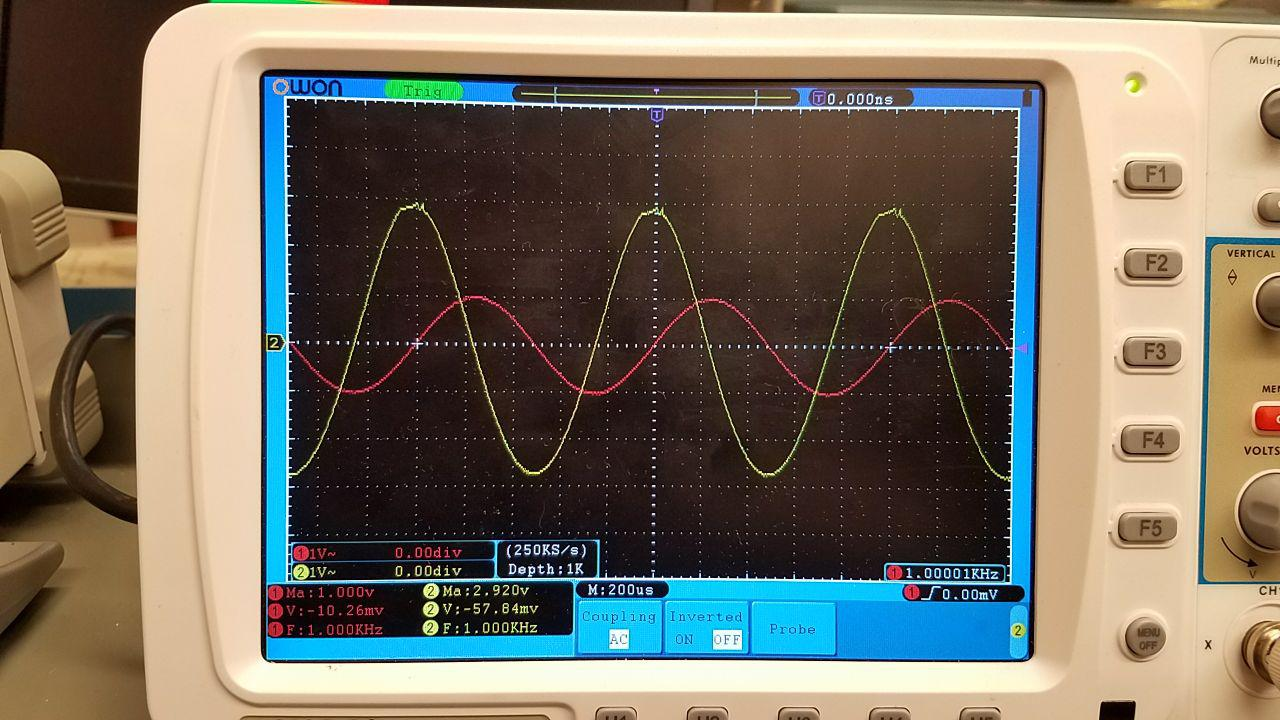
\includegraphics[width=\columnwidth]{IntegratorSine.eps}
	\caption{\label{integrator:sine}Integrator circuit with sinusoidal input.}
	\end{figure}

	\begin{figure}[H]
	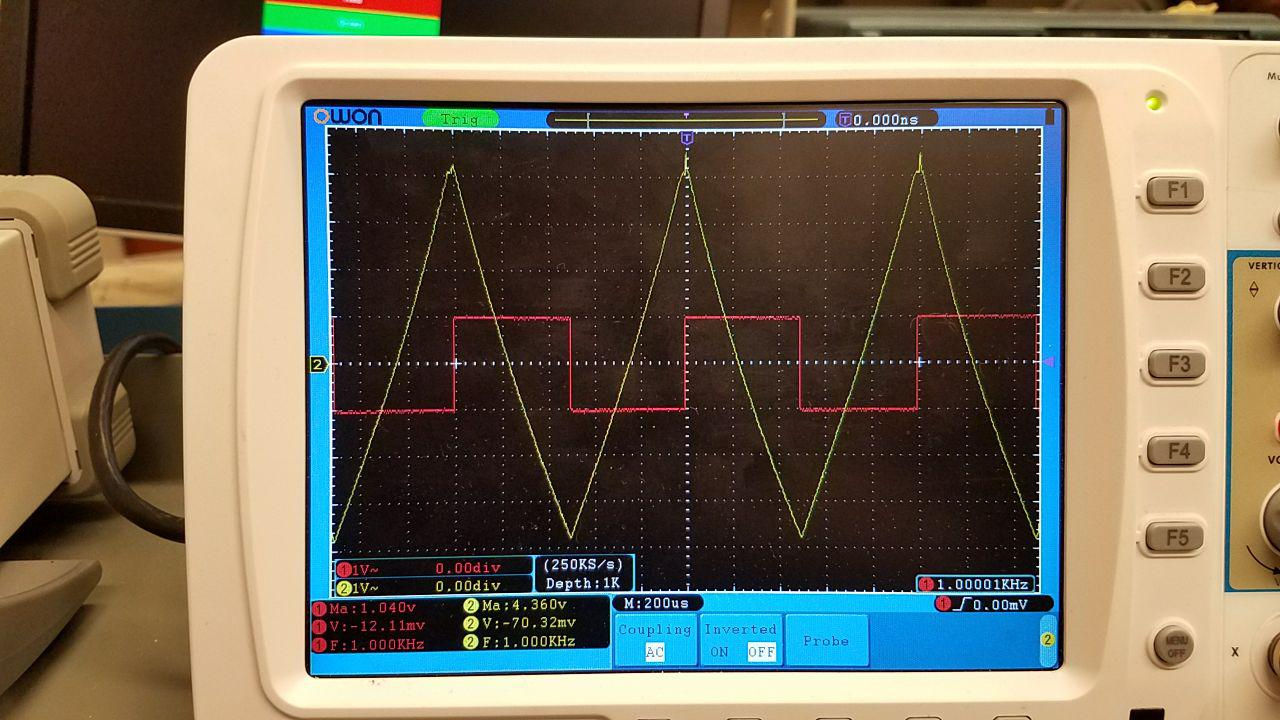
\includegraphics[width=\columnwidth]{IntegratorSquare.eps}
	\caption{\label{integrator:square}Integrator circuit with square input.}
	\end{figure}
		
	\begin{figure}[H]
	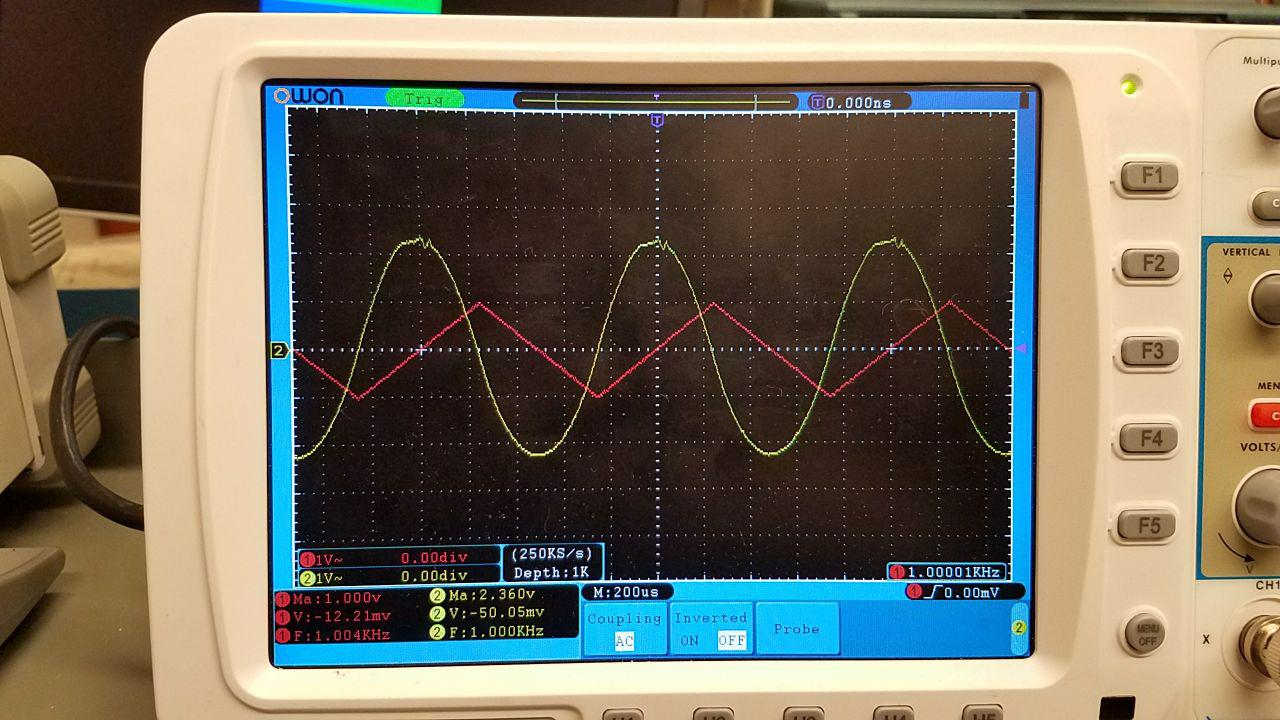
\includegraphics[width=\columnwidth]{IntegratorTriangle.eps}
	\caption{\label{integrator:triangle}Integrator circuit with triangle input.}
	\end{figure}		
	
	\subsection{5-7: Differentiator}
	
	\begin{figure}[H]
	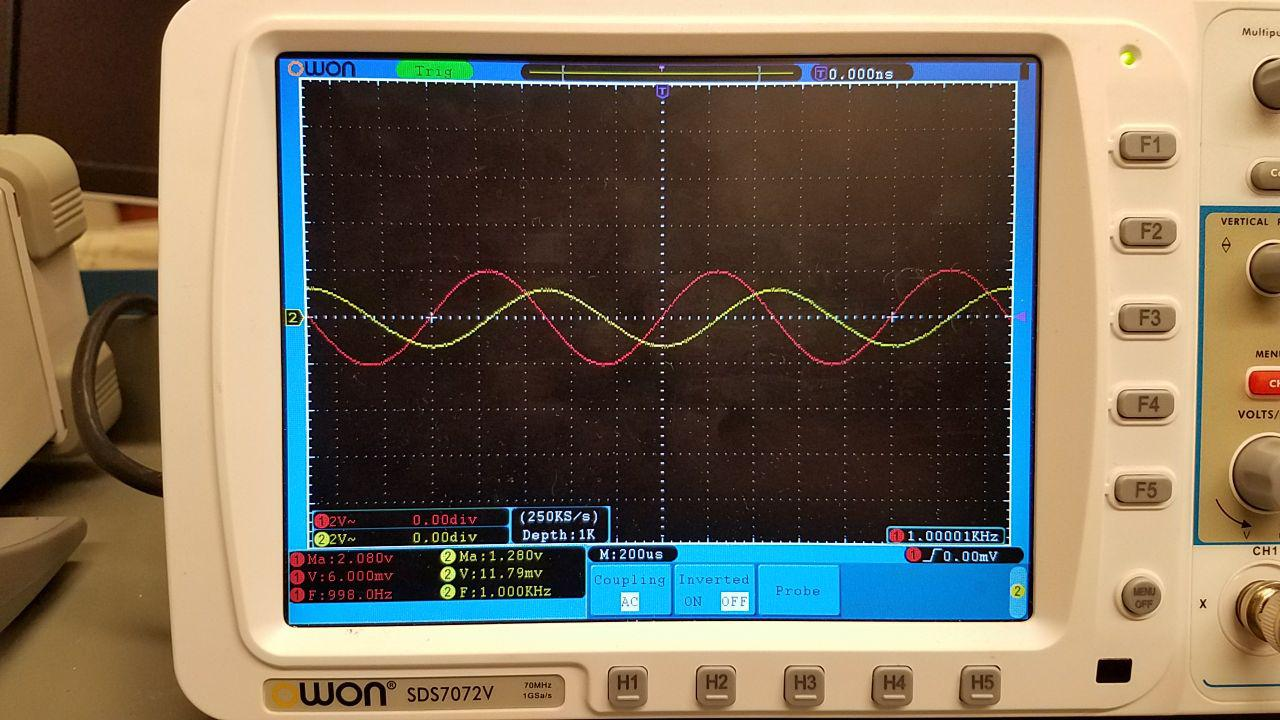
\includegraphics[width=\columnwidth]{DifferentiatorSine.eps}
	\caption{\label{differentiator:sine}Differentiator circuit with sinusoidal input.}
	\end{figure}

	\begin{figure}[H]
	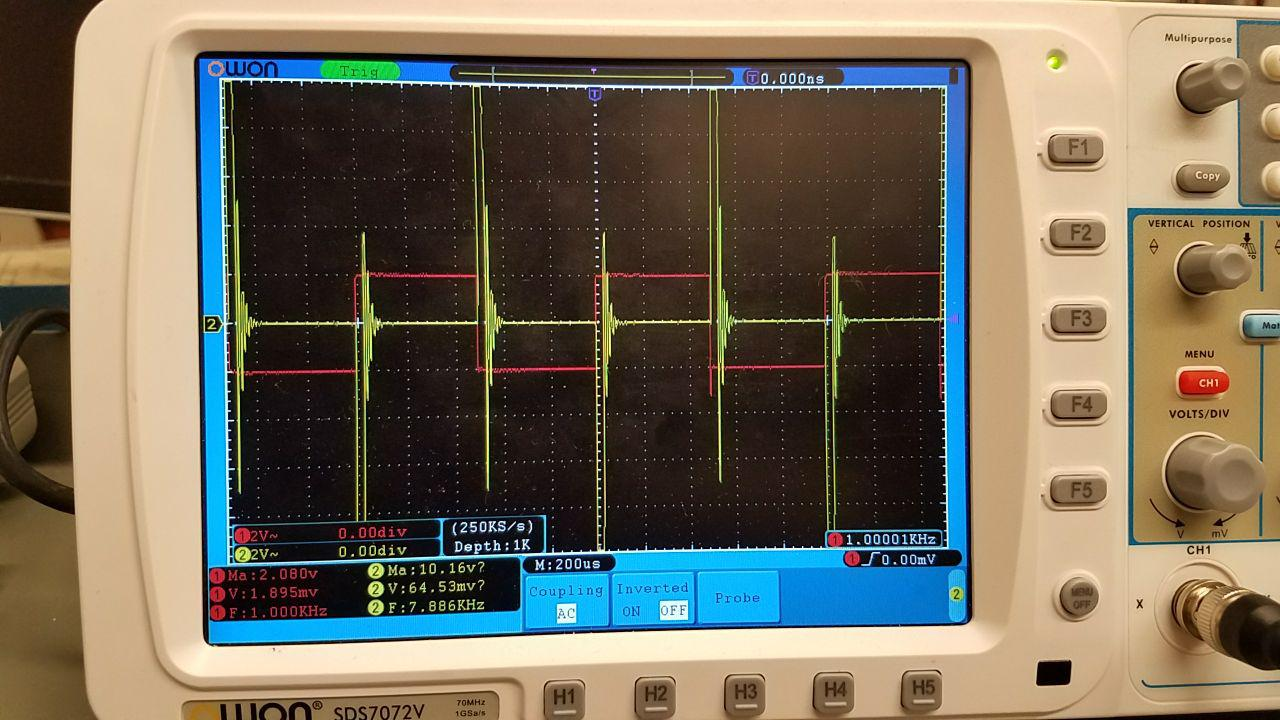
\includegraphics[width=\columnwidth]{DifferentiatorSquare.eps}
	\caption{\label{differentiator:square}Differentiator circuit with square input.}
	\end{figure}
		
	\begin{figure}[H]
	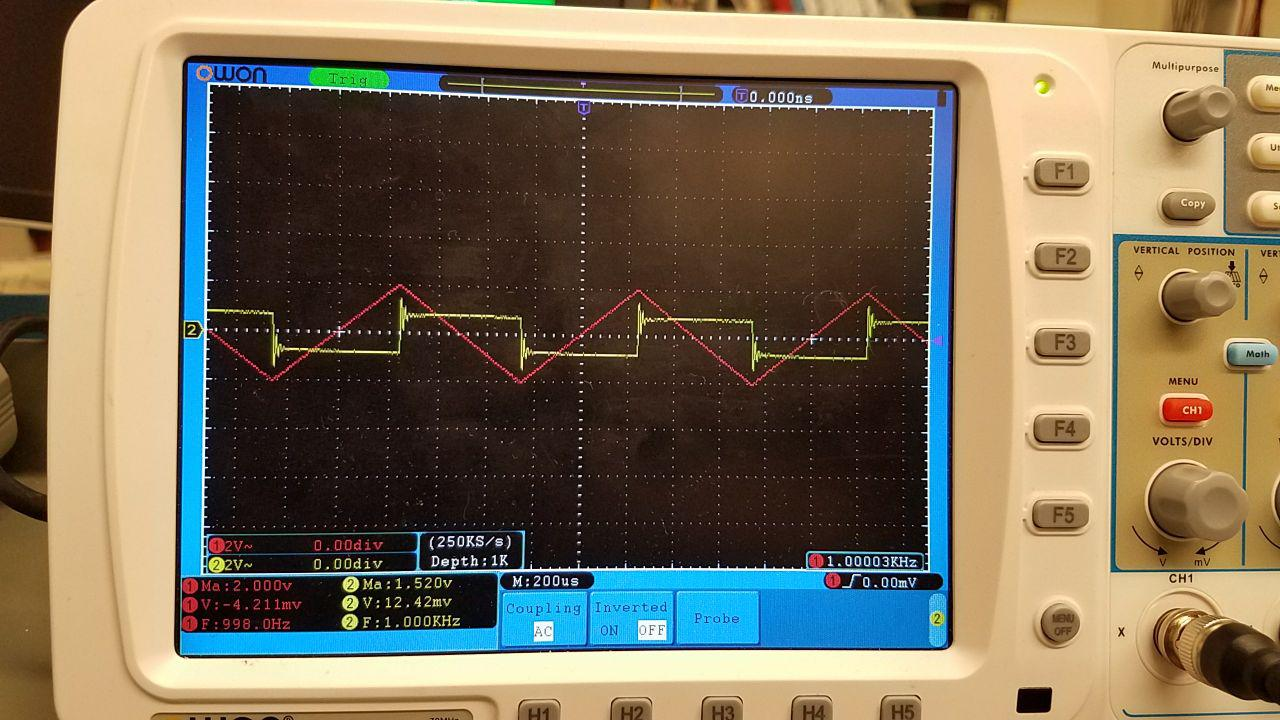
\includegraphics[width=\columnwidth]{DifferentiatorTriangle.eps}
	\caption{\label{differentiator:triangle}Differentiator circuit with triangle input.}
	\end{figure}		
	
	\subsection{5-8: Logarithmic Amplifier}
	
	\begin{tabularx}{0.45\textwidth}[t]{| X | X | X |}
	\hline
	\multicolumn{1}{|c|}{$V_{in}$} & \multicolumn{1}{|c|}{$ln(V_{in})$} & \multicolumn{1}{c|}{$V_{out}$}\\ \hline
	0.016 & -4.135 & -0.540\\ \hline
	0.360 & -1.022 & -0.600\\ \hline
	0.664 & -0.409 & -0.620\\ \hline
	0.960 & -0.041 & -0.620\\ \hline
	1.760 & 0.565 & -0.657\\ \hline
	5.000 & 1.609 & -0.683\\ \hline
	7.053 & 1.953 & -0.693\\ \hline
	9.903 & 2.293 & -0.701\\ \hline
	12.00 & 2.485 & -0.706\\ \hline
	\end{tabularx}
	
	\begin{tabularx}{0.45\textwidth}[t]{| X | X |}
	\hline
	\multicolumn{1}{|c|}{Slope} & \multicolumn{1}{c|}{y-intercept}\\ \hline
	-0.0249 & -0.630 \\ \hline
	\end{tabularx}
	
	\begin{figure}[H]
	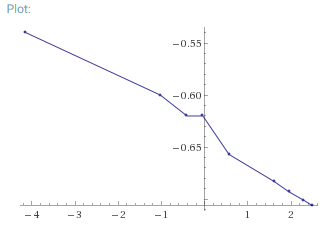
\includegraphics[width=\columnwidth]{logplot.eps}
	\caption{\label{logplot}plot of $ln(V_{in})$ vs $V_{out}$.}
	\end{figure}
	

\section{Discussion} \label{Section:Discussion}

	\subsection{5-1: Null Measurements}
	
	For experiment 5-1, there were a few things to notice. First is that depending on what side (side one or side two) of the TL082 we 
	were using, we had a different high/low rail. Side one's low rail was positive. Since we were using the inverted input, if you have a
	negative variable voltage input, your output will always be positive at full rail. When the circuit is at zero input, you get the full
	low rail. When you put a negative voltage into the inverted input, it tries to invert it (to positive) and gives you the full low rail.
	So you don't see much of a change.
	
	When using a positive variable voltage supply, it doesn't take much to make the circuit output the value of the negative rail at full. This
	makes sense when you consider later the behavior of the voltage comparator. We just need to get above a 0V value, and then this gives us our
	full rail. Because the lab equipment is not very sensitive, it was difficult to get an output that was less than 5mV. So the moment we touched
	the dial for the variable voltage supply, we would get negative full rail right away. 
	
	\subsection{5-2: Voltage Comparator}
	
	The voltage comparator on the other hand has a lot more practical applications. This circuit gave us a cutoff voltage at which point we get
	the full value of our +5V input once we've reached a threshold. This value for our circuit and components came out to a +5.36V minimum to get
	an output of +5.045V. When the input voltage of our variable voltage supply was below this value, we ended up getting 0.225V as a base output.
	
	As an aside, using a negative voltage input for our variable voltage supply on the non-inverting pin gave us nothing. Since the voltage never gets
	above +5.0V, the value never changed.
	
	When we connected the input voltage to a function generator, we started to see inconsistencies with the output frequencies when we went below
	39kHz and above 226kHz.
	
	\subsection{5-3: Voltage Follower}
	
	Due to there being no resistance in the circuit (and it seems that the resistivity of the wires themselves
	had no substantial value), what we ended up with, is a circuit that followed our input voltage with its output voltage, until it hit the maximum
	of what your VCC+ input was. For us, this value was always 11.40V
	
	\subsection{5-4: Follower with Gain}
	
	I stated in the Procedure section above that I failed to follow the directions of this lab, but I can at least comment on the results. We did get
	the gain values that we were expecting ($Gain = \frac{R_f}{R_{in}} + 1$). There was not much deviation from the expected values. A lot of the
	deviations we saw were due to the lack of stability in our voltage source, especially at low voltages. Anything below $\pm$1V, the input would
	fluctuate a bit, and since there was gain involved (and output lag) this would cause small deviations in our output.
	
	The percentage error of the offset voltage for the gain of 100 was negligible. In fact,
	since the output voltage was limited to 11.40V, if our input voltage was 0.2V (our lowest value of measure) our output voltage was stuck at 11.40V.
	This meant that for all measurements of the 100 gain circuit, our output was always 11.40V, due to the restrictions of our bipolar supply. 
	
	\subsection{5-5: Inverting Amplifier}
	
	The expected output for gain on the Inverting Amplifier is a little bit more simple ($Gain = -\frac{R_f}{R_{in}}$). Our error rate for the 100k$\Omega$
	was roughly 0.8\%. This difference was higher when we went to lower voltages (on the order of 10 millivolts). For the 10M$\Omega$ circuit, it was hard to
	gauge the error rate, as anything above 100mV would give us our full rail value (-10.80V to 11.40V). 
	
	\subsection{5-6: Integrator}
	
	When you integrate a linear function, you get a quadratic function, so the output looks almost sinusoidal. One thing that was noted as well was the lag that gave a phase angle to 
	the output. Looking at FIG. 2, FIG. 3, and FIG. 4, we saw a half wave length lag which is easiest to notice with the square wave. When the values are positive,
	the output should be increasing, but it is decreasing. This leads me to believe that the lag in the circuit gives a phase angle of $-\pi$. 
	
	\subsection{5-7: Differentiator}
	
	Much like the integrator circuit, we also see a phase angle of $-\pi$. What's interesting is not the sinusoidal waves, but the triangular and square waves.
	These functions are not differentiable. You can not take the derivative of a vertical line, or for a corner. What we see here in these circuits is almost a
	discontinuity with the outputs. For the square wave, we got a huge spike where the square wave changes. The capacitor acts as a spring, or a restoring force
	in these situations, which is why we saw it takes a moment to bounce back to a stable value. The triangle wave does this as well, but the magnitude of this
	spike is far less than the square wave.
	
	\subsection{5-8: Logarithmic Amplifier}
	
	The logarithmic amplifier does exactly what it says. It amplifies the circuit using a natural log. What we see when we use different input values, and look
	at the output values, is we get a function that is linear when we plot the natural log of the input versus the output. The equation we get for this is
	$y = -0.0249x - 0.630$.

\section{Conclusion}

The operational amplifier is a versatile, abstracted circuit that lets you harness the power of many mathematical functions simply based on components added to the circuit,
and changing our inputs. From a minimum value comparator, to an amplifier, negative amplifier, integrator, differentiator, and natural log amplifier, we have many mathematical
functions we can use to meet our needs. When we consider the power behind this concept (a simple circuit design letting us get the area underneath the curve of our input,
or letting us see the rate of change of our input), we begin to realize how powerful this small, higher level abstraction chip is.

The biggest drawback to the lab is the limitations of our input devices (the Elenco variable power supply is not sensitive enough to really give us accurate readings when we're
in the millivolts range). Beyond that, is our VCC+ and VCC- being low for our 100 Gain circuits. Almost any input you have on these circuits, you're limited to the full rail values
of the VCC+ and VCC-, so the different measurements become a moot point.

\end{document}